%
% $RCSfile: cybernetics_oriented_language.tex,v $
%
% Copyright (c) 2001-2004. Christian Heller. All rights reserved.
%
% No copying, altering, distribution or any other actions concerning this
% document, except after explicit permission by the author!
% At some later point in time, this document is planned to be put under
% the GNU FDL license. For now, _everything_ is _restricted_ by the author.
%
% http://www.cybop.net
% - Cybernetics Oriented Programming -
%
% http://www.resmedicinae.org
% - Information in Medicine -
%
% @author Christian Heller <christian.heller@tuxtax.de>
%

\section{Cybernetics Oriented Language}
\label{cybernetics_oriented_language_heading}

The introduced \emph{Cybernetics Oriented Language} (CYBOL) is based on the
principles of \emph{Human Thinking} as described in section \ref{human_thinking_heading}.
These principles and further concepts behind are summarized by the name
\emph{Cybernetics Oriented Programming} (CYBOP) (figure \ref{cybop_figure}).
They form the semantics of CYBOL. Its syntax is determined by the \emph{Extensible
Markup Language} (XML) standard and accordingly easy. It is rich enough to express
models based upon the three kinds of abstraction: \emph{Discrimination},
\emph{Categorization} and \emph{Composition} as well as meta information of a
\emph{Whole} about its \emph{Parts}.

\begin{figure}[ht]
    \begin{center}
        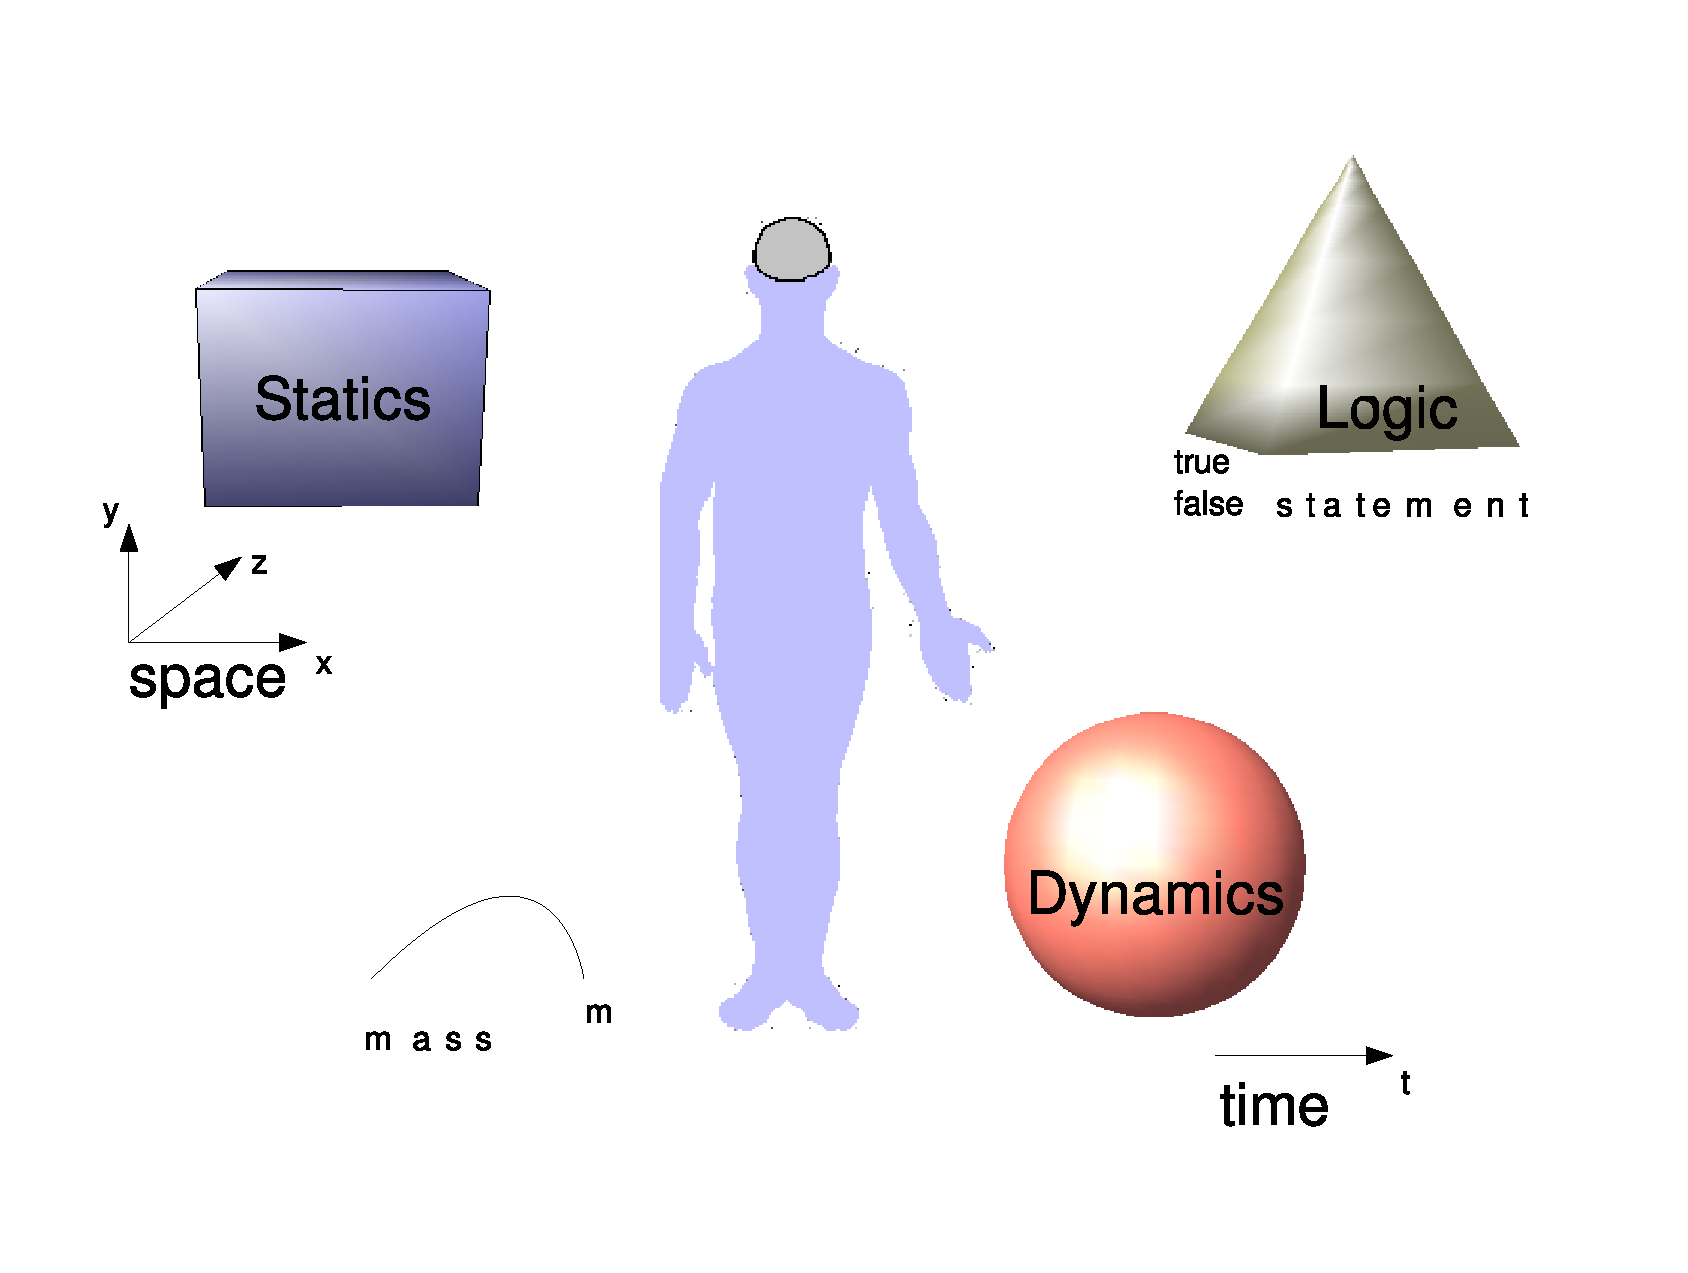
\includegraphics[scale=0.3]{vector/cybop.eps}
        \caption{CYBOP}
        \label{cybop_figure}
    \end{center}
\end{figure}

%
% $RCSfile: syntax.tex,v $
%
% Copyright (C) 2002-2008. Christian Heller.
%
% Permission is granted to copy, distribute and/or modify this document
% under the terms of the GNU Free Documentation License, Version 1.1 or
% any later version published by the Free Software Foundation; with no
% Invariant Sections, with no Front-Cover Texts and with no Back-Cover
% Texts. A copy of the license is included in the section entitled
% "GNU Free Documentation License".
%
% http://www.cybop.net
% - Cybernetics Oriented Programming -
%
% http://www.resmedicinae.org
% - Information in Medicine -
%
% Version: $Revision: 1.1 $ $Date: 2008-08-19 20:41:09 $ $Author: christian $
% Authors: Christian Heller <christian.heller@tuxtax.de>
%

\subsection{Syntax}
\label{syntax_heading}
\index{CYBOL Syntax}
\index{Syntax of a Language}
\index{Grammar of a Language}
\index{Extensible Markup Language}
\index{XML}
\index{XML Tag}
\index{XML Attribute}
\index{Discrimination}
\index{Composition}

Every language has a special \emph{Syntax}, that is a \emph{Grammar} with rules
for combining terms and symbols \cite{foldoc}. CYBOL could define its own
syntax or use an already existing one, of another language. Because of its
popularity, clear text representation, flexibility, extensibility and ease of
use, \emph{XML} was chosen to deliver the syntax for CYBOL.

To mention just two of the syntactical elements of XML, \emph{Tag} and
\emph{Attribute} are considered shortly here. Tags are special, arbitrary
keywords that have to be defined by the system working with an XML document.
Attributes keep additional information about the contents enclosed by two tags.
Two examples:

\begin{scriptsize}
    \begin{verbatim}
    <tag attribute="value">
        contents
    </tag>
    \end{verbatim}
\end{scriptsize}

\begin{scriptsize}
    \begin{verbatim}
    <tag attribute1="value" attribute2="contents"/>
    \end{verbatim}
\end{scriptsize}

An XML document carries a name and can such represent a \emph{Discrete Item},
as suggested by the principles of human thinking (section
\ref{human_thinking_heading}). Being a \emph{Compound}, it consists of parts --
and, it can link to other documents treated as its parts. That way, a whole
hierarchy can be formed. Tag attributes can keep additional information about
the linked parts. Most importantly, XML documents have a hierarchical structure
based on tags, which may be used to store meta information about a part.

Considering these properties of XML, it seems predestinated for formally
representing abstract models using the CYBOP concepts. CYBOL, finally, is XML
\emph{plus} a defined set of tags, attributes and values, used to structure and
link documents meaningfully.

%
% $RCSfile: vocabulary.tex,v $
%
% Copyright (c) 2001-2004. Christian Heller. All rights reserved.
%
% No copying, altering, distribution or any other actions concerning this
% document, except after explicit permission by the author!
% At some later point in time, this document is planned to be put under
% the GNU FDL license. For now, _everything_ is _restricted_ by the author.
%
% http://www.cybop.net
% - Cybernetics Oriented Programming -
%
% http://www.resmedicinae.org
% - Information in Medicine -
%
% @author Christian Heller <christian.heller@tuxtax.de>
%

\subsection{Vocabulary}
\label{vocabulary_heading}

XML allows to define and exchange the whole vocabulary of a language. It offers
two ways in which a list of legal elements can be defined: The traditional
\emph{Document Type Definition} (DTD) and the more modern \emph{XML Schema
Definition} (XSD). Besides the vocabulary, DTD and XSD define the structure of
an XML document and allow to typify, constrain and validate items. The CYBOL DTD
and XSD can be found at \cite{cybop}.

%
% $RCSfile: semantics.tex,v $
%
% Copyright (c) 2002-2007. Christian Heller. All rights reserved.
%
% Permission is granted to copy, distribute and/or modify this document
% under the terms of the GNU Free Documentation License, Version 1.1 or
% any later version published by the Free Software Foundation; with no
% Invariant Sections, with no Front-Cover Texts and with no Back-Cover
% Texts. A copy of the license is included in the section entitled
% "GNU Free Documentation License".
%
% http://www.cybop.net
% - Cybernetics Oriented Programming -
%
% Version: $Revision: 1.1 $ $Date: 2007-08-01 13:59:00 $ $Author: christian $
% Authors: Christian Heller <christian.heller@tuxtax.de>
%

\section{Semantics}
\label{semantics_heading}
\index{Semantics}
\index{State Knowledge Modelling}
\index{Logic Knowledge Modelling}
\index{Extensible Markup Language}
\index{XML}
\index{XML Tag}
\index{XML Attribute}

The meaning expressed by terms and sentences is their \emph{Semantics}
\cite{duden}.

CYBOL files can be used to model \emph{State Knowledge} (like a graphical
window or a person's address) and \emph{Logic Knowledge} (like an operation or
algorithm or workflow) \cite{cybopbook}. In both cases, the \emph{same} syntax
(document structure) with \emph{identical} vocabulary (XML tags and -attributes)
is applied. It is the attribute \emph{Values} that make a difference in meaning.

The double hierarchy mentioned before is realised in CYBOL knowledge templates
by using XML \emph{Attributes} for representing the whole-part hierarchy, and
XML \emph{Tags} for representing the additional meta data that a whole model
keeps about its part models.

%
% $RCSfile: attributes.tex,v $
%
% Copyright (C) 2002-2008. Christian Heller.
%
% Permission is granted to copy, distribute and/or modify this document
% under the terms of the GNU Free Documentation License, Version 1.1 or
% any later version published by the Free Software Foundation; with no
% Invariant Sections, with no Front-Cover Texts and with no Back-Cover
% Texts. A copy of the license is included in the section entitled
% "GNU Free Documentation License".
%
% http://www.cybop.net
% - Cybernetics Oriented Programming -
%
% http://www.resmedicinae.org
% - Information in Medicine -
%
% Version: $Revision: 1.1 $ $Date: 2008-08-19 20:41:05 $ $Author: christian $
% Authors: Christian Heller <christian.heller@tuxtax.de>
%

\subsubsection{Attributes}
\label{attributes_heading}
\index{CYBOL Attributes}
\index{CYBOL 'name' Attribute}
\index{CYBOL 'channel' Attribute}
\index{CYBOL 'abstraction' Attribute}
\index{CYBOL 'model' Attribute}

Normally, an XML \emph{Attribute} keeps meta information about the contents of
an XML \emph{Tag}. In CYBOL, however, three attributes keep meta information
about a fourth attribute. The attributes, altogether, are:

\begin{itemize}
    \item[-] name
    \item[-] channel
    \item[-] abstraction
    \item[-] model
\end{itemize}

The attribute of greatest interest is \emph{model}. It contains a model either
directly, or a path to one. The \emph{channel} attribute indicates whether the
\emph{model} attribute's value is to be read from:

\begin{itemize}
    \item[-] inline
    \item[-] file
    \item[-] ftp
    \item[-] http
\end{itemize}

The \emph{abstraction} attribute specifies how to interpret the model pointed
to by the \emph{model} attribute's value. A model may be given in formats like
for example:

\newpage

\begin{itemize}
    \item[-] cybol (a state- or logic compound model encoded in CYBOL format)
    \item[-] operation (a primitive logic model)
    \item[-] string
    \item[-] double
    \item[-] integer
    \item[-] boolean
\end{itemize}

The \emph{name} attribute, finally, provides the referenced model with a unique
identifier.

While the interpretation of the \emph{model} attribute's value depends on the
\emph{channel-} and \emph{abstraction} attributes, the other three attributes
(\emph{name}, \emph{channel}, \emph{abstraction}) themselves always get
interpreted as character string.

%
% $RCSfile: tags.tex,v $
%
% Copyright (C) 2002-2008. Christian Heller.
%
% Permission is granted to copy, distribute and/or modify this document
% under the terms of the GNU Free Documentation License, Version 1.1 or
% any later version published by the Free Software Foundation; with no
% Invariant Sections, with no Front-Cover Texts and with no Back-Cover
% Texts. A copy of the license is included in the section entitled
% "GNU Free Documentation License".
%
% http://www.cybop.net
% - Cybernetics Oriented Programming -
%
% http://www.resmedicinae.org
% - Information in Medicine -
%
% Version: $Revision: 1.1 $ $Date: 2008-08-19 20:41:09 $ $Author: christian $
% Authors: Christian Heller <christian.heller@tuxtax.de>
%

\subsubsection{Tags}
\label{tags_heading}
\index{CYBOL Tags}
\index{CYBOL 'model' Tag}
\index{CYBOL 'part' Tag}
\index{CYBOL 'property' Tag}
\index{CYBOL 'constraint' Tag}

There are many kinds of meta information besides the above-mentioned
attributes, that may be known about a model. These are given in special XML
tags called \emph{property} and \emph{constraint}. As defined in section
\ref{vocabulary_heading}, a CYBOL knowledge template may use four kinds of XML
tags:

\begin{itemize}
    \item[-] model
    \item[-] part
    \item[-] property
    \item[-] constraint
\end{itemize}

The \emph{model} tag appears just once. It is the root node which makes a CYBOL
knowledge template a valid XML document.

Of actual interest are the \emph{part} tags. They identify the models that the
\emph{whole} model described by the CYBOL knowledge template consists of.

A \emph{whole} model may know a lot more about its \emph{part} models, than is
given by a part model's XML attributes. A spatial state model may know about
the \emph{position} and \emph{size} of its parts, in space. A temporal model
(such as a workflow) may have to know about the \emph{position} of its parts in
time, in order to be able to execute them in the correct order. Further, the
temporal model needs to know about the \emph{input/output} (i/o) state models
which are to be manipulated by the corresponding logic operation (part model).
The number of parts within a whole (compound) model may be limited. And so on.
These additional information are provided by \emph{property} tags whose number
is conceptually unlimited.

Not only parts need additional meta information; properties may need such
information, too. The position or size as properties of a part may have to be
constrained to certain values, such as a \emph{minimum} or \emph{maximum}. The
values of the \emph{colour} property of a part model may have to be chosen out
of a pre-defined set called \emph{choice}. Information of that kind are stated
in \emph{constraint} tags.

Since the number of possible meta information implementable in CYBOL is already
quite large and steadily growing, as the development continues, this section
cannot list them all. At a future point in time, a more-or-less complete CYBOL
specification document may be found at the CYBOP project's website \cite{cybop}.

%
% $RCSfile: tag_attribute_swapping.tex,v $
%
% Copyright (C) 2002-2008. Christian Heller.
%
% Permission is granted to copy, distribute and/or modify this document
% under the terms of the GNU Free Documentation License, Version 1.1 or
% any later version published by the Free Software Foundation; with no
% Invariant Sections, with no Front-Cover Texts and with no Back-Cover
% Texts. A copy of the license is included in the section entitled
% "GNU Free Documentation License".
%
% http://www.cybop.net
% - Cybernetics Oriented Programming -
%
% http://www.resmedicinae.org
% - Information in Medicine -
%
% Version: $Revision: 1.1 $ $Date: 2008-08-19 20:41:09 $ $Author: christian $
% Authors: Christian Heller <christian.heller@tuxtax.de>
%

\subsection{Tag-Attribute Swapping}
\label{tag_attribute_swapping_heading}
\index{CYBOL Tag-Attribute Swapping}

CYBOL swaps the meaning attributes and tags traditionally have in XML
documents, where tags represent elements that may be nested infinitely and
attributes hold additional (meta) information about a tag. Following an example
of how CYBOL might have looked that way:

\begin{scriptsize}
    \begin{verbatim}
<model>
    <part>
        <name="title"/>
        <channel="inline"/>
        <abstraction="character"/>
        <model="Res Medicinae"/>
    </part>
    <part layout="compass" position="north">
        <name="menu_bar"/>
        <channel="file"/>
        <abstraction="cybol"/>
        <model="gui/menu_bar.cybol"/>
    </part>
</model>
    \end{verbatim}
\end{scriptsize}

The current final specification of CYBOL, on the contrary, uses attributes to
define a nested element (part) and tags to give properties (meta information)
about such a nested element, in the following way:

\begin{scriptsize}
    \begin{verbatim}
<model>
    <part name="title" channel="inline" abstraction="character" model="Res Medicinae"/>
    <part name="menu_bar" channel="file" abstraction="cybol" model="gui/menu_bar.cybol">
        <property name="layout" channel="inline" abstraction="character" model="compass"/>
        <property name="position" channel="inline" abstraction="character" model="north"/>
    </part>
</model>
    \end{verbatim}
\end{scriptsize}

This is because:

\begin{enumerate}
    \item the number of attributes specifying a part in CYBOL is fixed, whereas
        the number of tags specifying a property of a part is not, and the
        number of XML tags is easier extensible than that of attributes;
    \item that way it is also possible to specify a part without any properties
        in just one CYBOL code line, while otherwise four tags would always
        have to be given;
    \item not only a part may be nested (consist of smaller parts), but also a
        property may be (for example a position consisting of three coordinates
        given as parts), which necessitates the four standard attributes to be
        given for properties and constraints as well.
\end{enumerate}


%
% $RCSfile: example.tex,v $
%
% Copyright (c) 2001-2004. Christian Heller. All rights reserved.
%
% No copying, altering, distribution or any other actions concerning this
% document, except after explicit permission by the author!
% At some later point in time, this document is planned to be put under
% the GNU FDL license. For now, _everything_ is _restricted_ by the author.
%
% http://www.cybop.net
% - Cybernetics Oriented Programming -
%
% http://www.resmedicinae.org
% - Information in Medicine -
%
% @author Christian Heller <christian.heller@tuxtax.de>
%

\subsection{Example}
\label{example_heading}

The following example shows a minimalistic model of a (static) \emph{Graphical
User Interface} (GUI) frame.

\begin{verbatim}
<!--
    frame_example.cybol
/-->
<model>
    <part name="title"
        part_abstraction="string"
        part_model="Res Medicinae"/>
    <part name="menu_bar"
        part_abstraction="compound"
        part_model="/gui/menu_bar.cybol"
        position_abstraction="compass"
        position_model="north"/>
    <part name="status_bar"
        part_abstraction="compound"
        part_model="/gui/tool_bar.cybol"
        position_abstraction="compass"
        position_model="south"/>
</model>
\end{verbatim}

Similar models can be built of (dynamic) workflows whereby the inputs and outputs
of the part operations appear in a special order as attribute values. But this
may become the topic of a follow-up paper.

